% 3006ICT Group Project -- Final Report (ICCV 2025 template, camera-ready)
\documentclass[10pt,twocolumn,letterpaper]{article}

%%%%%%%%% PAPER TYPE
\usepackage{iccv}              % To produce the CAMERA-READY version
% \usepackage[review]{iccv}      % To produce the REVIEW version
% \usepackage[pagenumbers]{iccv} % To force page numbers, e.g. for an arXiv version

% Packages and macros loaded after iccv.sty (before hyperref).
\usepackage{array}  % >{...} column specifiers in the tables

% bold run-in paragraph leads
\newcommand{\lead}[1]{\par\smallskip\noindent\textbf{#1}\hspace{0.4em}}


\definecolor{iccvblue}{rgb}{0.21,0.49,0.74}
\usepackage[pagebackref,breaklinks,colorlinks,allcolors=iccvblue]{hyperref}

\def\paperID{*****}
\def\confName{3006ICT}
\def\confYear{2026}

%%%%%%%%% TITLE
\title{Autonomous Visual Object Finding with an e-puck:\\
Perception, Route Planning and Safety}

%%%%%%%%% AUTHORS
\author{
SYUAN-HAO LI \quad Isaac Mangano \quad Hyunkyung Lee\\
Griffith University\\
{\small s5453352, syuan-hao.li@griffithuni.edu.au}\\
{\small s5418871, isaac.mangano@griffithuni.edu.au}\\
{\small s5432909, hyunkyung.lee@griffithuni.edu.au}
}

\begin{document}
\maketitle

\begin{abstract}
An e-puck robot in a known Webots arena must find which of eight stations shows a requested target object, and stop at that station's observation position within four minutes without collision. Which station displays the requested target must be determined from the robot's low-resolution $160{\times}120$ camera, which sees only the dark lower half of each poster. We combine three parts. A DINOv3 ViT-S/16 classifier is fine-tuned on the eight reference images with view-matched augmentation; it reaches 100\% accuracy on unseen station frames at near-square poses and runs in 32\,ms on a CPU. An A* planner visits stations in greedy nearest-first order on the supplied occupancy grid. A two-layer safety monitor combines directional proximity checks with progress-based stuck detection. Scored by an independent referee, the final controller completes all three provided student missions (130--162\,s) and all 192 missions of an expanded benchmark of 3 starts $\times$ 8 targets $\times$ 8 cyclic station layouts, in which every target appears at every station (median 73\,s, worst 162\,s), with no collision and a median stopping error of 3.7\,cm. Benchmark performance was unchanged when the camera scan was removed or the start pose was perturbed. In a deliberately introduced unmapped-obstacle test, the safety monitor raised success from 0\% to 59\%, and its remaining failures point to two concrete fixes.
\end{abstract}

\section{Introduction}
\label{sec:intro}

% Rubric: problem understanding, project idea and design rationale (8)
The task is simulated in Webots~\cite{michel2004webots} with an e-puck robot~\cite{mondada2009epuck}. \TODO{The problem: an e-puck in a known arena with eight observation stations; one station displays the mission target. Success = stopping within 0.20\,m of the correct observation position, no collision, within 4:00 simulation time.}

\TODO{What makes it hard: target identity is only available visually (no world-file or texture access); low camera sees only the lower half of each poster; several stations are in shadow; robot arrives with heading error; narrow corridors.}

\TODO{Project idea in one paragraph: map-based navigation to candidate stations + visual verification at each station + two-layer safety monitor.}

\paragraph{Contributions.}
\begin{itemize}[nosep]
  \item \TODO{Perception: DINOv3 ViT-S/16 fine-tuned on eight reference images with view-matched augmentation; 32\,ms/frame on CPU.}
  \item \TODO{Planning: grid-based shortest-path planning and nearest-station visiting order.}
  \item \textbf{Safety:} A two-layer safety monitor combining per-step directional proximity monitoring with progress-based stuck detection for contacts missed by the proximity sensors, with replanning after each safety event. 
  The front thresholds were empirically calibrated, improving stopping clearance in a 45$^\circ$ approach from 3.6\,cm to 5.2\,cm, and the stuck detector was validated through fault-injection tests. (\cref{sec:safety})
  \item \TODO{Evaluation: three student missions plus a 96-run Monte Carlo benchmark with an independent referee.}
\end{itemize}

\section{System Overview}
\label{sec:system}

\begin{figure}[t]
  \centering
  \figholder{Pipeline diagram: mission json $\rightarrow$ station order $\rightarrow$ plan $\rightarrow$ drive (safety loop) $\rightarrow$ scan \& classify $\rightarrow$ stop / next station}{4cm}
  \caption{System overview. \TODO{caption}}
  \label{fig:overview}
\end{figure}

\TODO{Mission flow (\cref{fig:overview}): read target label; pick nearest unvisited station; plan and drive to its observation cell; turn to observation yaw; classify; stop if match, otherwise continue.}

\TODO{Sensors and what each is used for (camera: target identity only; GPS/IMU + map: localisation and navigation; ps0--ps7: safety). State explicitly what is \emph{not} used (world files, texture URLs, ground truth).}

\TODO{Code structure: \texttt{detector/}, \texttt{path/}, \texttt{robot/}, \texttt{safety/}, \texttt{stations/}; how the modules are integrated in the main loop.}

\section{Perception}
\label{sec:perception}
\owner{\TODO{Name}}

\subsection{Problem and design rationale}
\TODO{Eight known classes, one reference image each $\rightarrow$ few-shot classification. Constraints: CPU inference, run-time budget, domain gap between clean reference and low, dark, off-axis camera view.}

\subsection{Candidate approaches}
We compare vision-language models~\cite{radford2021clip} and self-supervised ViTs~\cite{dosovitskiy2021vit,simeoni2025dinov3}. \TODO{Compared zero-shot CLIP/SigLIP2, prototype matching on frozen features (CLIP, DINOv2, DINOv3, ResNet18, MobileNetV3), and full fine-tuning. Why prototypes fail (cosine margin $\approx$0.02).}

\begin{table}[t]
  \centering\small
  \begin{tabular}{@{}lccc@{}}
    \toprule
    Method & Normal & Hard & CPU ms \\
    \midrule
    Zero-shot CLIP            & \TODO{} & \TODO{} & \TODO{} \\
    Prototype (DINOv3-S)      & \TODO{} & \TODO{} & \TODO{} \\
    Fine-tune ResNet18        & \TODO{} & \TODO{} & \TODO{} \\
    Fine-tune DINOv3 ViT-S/16 & 100.0   & 88.7    & 32 \\
    \bottomrule
  \end{tabular}
  \caption{Encoder comparison on captured frames. \TODO{fill from perception report}}
  \label{tab:encoders}
\end{table}

\subsection{Method}
We fine-tune DINOv3 ViT-S/16~\cite{simeoni2025dinov3} from timm~\cite{wightman2019timm} with label smoothing~\cite{szegedy2016rethinking}. \TODO{DINOv3 ViT-S/16 (timm), CLS pooling, $224{\times}224$ whole-frame resize (no centre crop). View-matched augmentation: lower 40--70\% crop of the reference, brightness $0.3$--$0.8\times$, dark band below. Label smoothing; fp16 checkpoint (43\,MB).}

\subsection{Open-set rejection and multi-view scan}
\TODO{Confidence threshold 0.20 (distractor FPR@95 = 0\%). Scan at each station and keep the most confident frame; yaw error vs.\ accuracy curve.}

\begin{figure}[t]
  \centering
  \figholder{yaw error vs.\ accuracy (single frame / whole frame / multi-view) -- see \texttt{perception/report/figs/yaw\_curves.pdf}}{3.5cm}
  \caption{Accuracy against heading error. \TODO{caption}}
  \label{fig:yaw}
\end{figure}

\subsection{Perception results}
\TODO{Key findings: centre crop loses the poster at yaw error; whole-frame input recovers most of it; auto-crop adds little beyond that; scan reaches $\approx$100\% within $\pm30^\circ$.}

\section{Route Planning}
\label{sec:planning}

\subsection{Problem and design rationale}
Robot path planning can be done with many algorithms. Discrete methods such as Dijkstra~\cite{dijkstra1959note}, A*~\cite{hart1968astar} and Bellman-Ford search a graph; continuous sampling methods such as Rapidly-exploring Random Trees (RRT) and RRT* sample the free space. They trade off time complexity, space complexity, support for negative weights and optimality of the path.

In this project the arena is a known 2D map that fits a $40\times40$ grid, and the obstacles and observation stations are available to the program at run time. The station that shows the target, however, is unknown to the robot, so stations must be visited until the target is found. Navigation therefore reduces to repeated shortest-path queries on a known graph, followed by a visual check at each station.

\subsection{Map representation}
As mentioned, the obstacles and stations lie within a $40\times40$ grid at 0.1\,m per cell (385 occupied cells). The provided program includes a coordinate system and helpers that convert GPS positions to grid cells and back. The IMU yaw, rounded to the nearest multiple of $90^\circ$, gives the robot's grid heading. The planner rejects the two outermost rows and columns as a safety margin along the arena wall.

\subsection{Shortest path}
Given the problem and environment, we narrowed the choice to discrete methods, in particular Dijkstra and A*.

\lead{Why not sampling-based planners.} Sampling methods do not match the cell-based coordinate API we were given. They could arguably produce shorter paths, because they allow motion in any direction rather than the four directions and discrete cells we chose, but they are non-deterministic and need path smoothing. With the coordinate API and a generous 4-minute limit, we chose the simpler discrete approach. Incremental replanners such as D* Lite were also unnecessary: replanning happens only after a safety event, and a full replan takes well under a millisecond.

\lead{Why A*.} Among discrete methods we required a guaranteed shortest path. Depth-first search (DFS) gives no such guarantee and was excluded. Breadth-first search (BFS) does return shortest paths on our grid, where every move costs the same; in fact our Dijkstra on unit costs behaves like BFS with a priority queue. However, BFS stops being optimal as soon as moves have different costs, for example turn penalties or clearance costs, so we preferred a cost-based planner that extends to them. Bellman-Ford was ruled out because our costs are never negative, so its extra complexity buys nothing. Dijkstra and A* both return optimal paths when the A* heuristic never overestimates the true distance, which holds for the Manhattan distance on a 4-connected grid. We therefore chose between them by execution time (\cref{tab:planner-timing}).

\begin{table}[tbp]
  \centering\small
  \setlength{\tabcolsep}{4pt}
  \begin{tabular}{@{}lcccc@{}}
    \toprule
    Time (ms) & Mean & Median & Min & Max \\
    \midrule
    Dijkstra & 0.757 & 0.764 & 0.144 & 1.410 \\
    A*       & 0.208 & 0.153 & 0.026 & 0.767 \\
    \midrule
    Speed-up & \multicolumn{4}{c}{$3.65\times$ (by mean)} \\
    \bottomrule
  \end{tabular}
  \caption{Planner execution time over all 110 ordered start/station pairs on the $40\times40$ occupancy grid (25 repeats per pair, one CPU core). Both planners returned paths of identical, optimal length on every pair, and A* is 3.65$\times$ faster by mean time (median per-pair speed-up 4.2$\times$, range 1.7--10.3$\times$; \cref{app:planners}).}
  \label{tab:planner-timing}
\end{table}

As \cref{tab:planner-timing} shows, A* runs 3.65$\times$ faster than Dijkstra by mean time, and the per-pair median speed-up is 4.2$\times$. We therefore chose A*. Both planners finish in under a millisecond, while a mission takes 70--160\,s, so the speed-up has little effect on mission time. \Cref{app:planners} adds greedy best-first search, which is faster still but returns longer paths on 26 of 110 pairs, and a turn-penalised A* that keeps paths optimal while needing 47\% fewer turns.

\subsection{Station visiting order}
For the visiting order we chose a greedy nearest-neighbour rule. The planner keeps a list of all station coordinates and pops the nearest one (Manhattan distance from the robot's cell) as the next destination. TSP-style tours also exist, but the mission can end at any station before all have been visited, which makes nearest-neighbour search appealing. The resulting tours are fixed by the start position (\cref{fig:route}). Their cost shows in the student missions: from every start the target station S1 is reached only 7th or 8th, which sets their 130--162\,s mission times (\cref{fig:traj}).

We also considered an information-driven approach. An object detector would find station images anywhere in the robot's view, and stereo mapping would project each detection to world coordinates using the camera intrinsics and extrinsics, locating the station it belongs to. That station would then be removed from the list if it did not show the target, or visited directly if it did. However, the robot has no stereo or depth camera, so world coordinates cannot be recovered from a single detection.

\subsection{Motion execution}
Once a path is generated, the robot receives a list of discrete moves in the world frame. The problem then becomes turning a world direction such as ``UP'' into in-place rotations and forward moves. We solve it with rotation matrices: one for the desired global direction and one for the robot's current global direction. The goal is the rotation the robot must perform to face the desired direction.

This is similar to the extrinsic matrix in computer vision: we need the world direction as seen from the robot. The inverse of the robot's global direction serves as its extrinsic matrix. Multiplying it by the desired global direction gives that direction in the robot's frame, which is exactly the rotation the robot needs (straight, left, right or back).

Each forward move drives at full wheel speed until the GPS cell changes, while the safety layers (\cref{sec:safety}) monitor every simulation step. Each turn rotates in place until the IMU yaw is within 0.1\,rad of the next multiple of $90^\circ$. At the station, \texttt{go\_to\_yaw} turns the shorter way to the observation yaw, and the robot takes four frames at $\pm5^\circ$ and $\pm10^\circ$ for the classifier (\cref{sec:perception}). Raising the scan's wheel speed from 0.1 to 0.5\,rad/s, released together with the switch to A*, cut the worst-case mission time from 229\,s to 162\,s (\cref{tab:mc}).

\begin{figure*}[tbp]
  \centering
  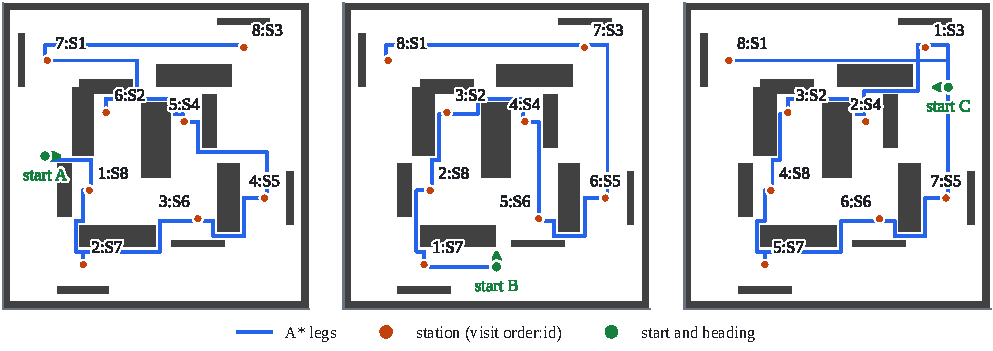
\includegraphics[width=\textwidth]{figs/route_planning.pdf}
  \caption{Greedy nearest-neighbour tours from (a) Start~A, (b) Start~B and (c) Start~C, produced by replaying the controller's station order and A* planner on the $40\times40$ occupancy grid (blue: A* legs between consecutive observation cells; labels: visit order and station; green arrow: start pose). The order is fixed by the start alone, and the mission stops at the first station showing the target, so mission time depends mainly on that station's position in the tour: S1, the student-mission target, comes 7th or 8th from every start.}
  \label{fig:route}
\end{figure*}

\section{Safety}
\label{sec:safety}
\owner{Hyunkyung Lee}

\subsection{Problem and design rationale}
Even a single collision causes a mission to fail. 
Our path planner uses an occupancy grid to generate a path that avoids obstacle cells, but it cannot account for heading errors, deviations in travel distance, and contact with or slippage along walls that occur during actual driving. 

Consequently, instead of making changes to the path planner itself, we created an additional monitoring layer---a safety function that observes the robot's actual state while the planned movement takes place. 
When danger is detected, the current movement is stopped immediately, and a safety event is returned to prompt the controller to replan the path from the current position.

There are two reasons why a monitoring-based approach is preferable to a reactive obstacle avoidance method. 
First, in a static assessment environment, since the global planner already provides a valid grid path, continuous reactive steering could disrupt the planned path and the discrete one-cell movement structure. 
Second, the monitoring layer does not change the navigation behaviour unless there is an anomaly and, since the checks are solely computational and Webots waits for the controller at every step, it does not add to the mission time.

The safety system consists of two complementary layers. 
The first layer uses proximity sensors to detect a dangerous approach to obstacles before a collision occurs. 
The second layer is a stuck detector that monitors actual movement and serves as a fallback mechanism to detect contact that the proximity sensors may have missed.

\subsection{Layer 1: directional proximity monitoring}
Proximity monitoring of four sensor groups (FRONT, RIGHT, BACK, LEFT; \cref{tab:safety_parameters}) is carried out at each simulation step (32\,ms) for each forward movement.
If one or more sensor groups exceed their threshold values, the movement stops immediately, resulting in a safety event being activated. 
To handle situations of simultaneous danger detection from different directions, a set is returned, representing the dangers detected. 
Proximity monitoring is not carried out when the robot performs a rotation on the spot because the robot's circular footprint means there is no difference in the distance of its center from any obstacles as it rotates in place. 

The front threshold was determined through a calibration test. 
Using a test-only controller (\texttt{safety\_diagnostic}), the robot was driven toward a wall at the same speed as in an actual mission; the sensor readings and distance traveled for each step were recorded until contact was made, and the remaining distance (clearance) for each step was calculated in reverse from the point of contact.
The peak values of all proximity sensors observed during normal full-mission operation (Start A/B/C) were 80.4 or lower. 
The initial front threshold of 80 lies within this noise range, which confirms that the current threshold of 120 is needed; it provides a sufficient margin between normal movement and dangerous proximity. 
The side threshold (150) and back threshold (120) remain at their initial values; while it was confirmed that there were no false positives during normal operation, unlike the front threshold, no separate calibration for clearance was performed. 

In the initial implementation, only ps0 and ps7 were used for detection of front dangers. However, during a calibration test involving an approach to a wall at a 45$^\circ$ angle, it was observed that the front-diagonal sensor ps6 exceeded the threshold before ps7 did. 
It was concluded that detection was delayed when using only ps0 and ps7 in approaching the wall at an angle; thus ps1 and ps6 were added as front-diagonal sensors. 
After this addition, the clearance at a stop during a 45$^\circ$ approach increased from 3.6\,cm to 5.2\,cm, while the clearance during a head-on approach remained at the original 2.5\,cm. 

If only a FRONT danger is detected, the robot verifies whether the back sensors indicate a safe condition and then performs a brief reverse recovery, and continues to monitor for BACK proximity even while reversing. 
In the case of LEFT, RIGHT, or BACK danger, the robot does not perform a separate reactive avoidance manoeuvre. 

\begin{table}[tbp]
\centering
\footnotesize
\setlength{\tabcolsep}{3pt}
\begin{tabular}{@{}>{\raggedright\arraybackslash}p{2.2cm}>{\raggedright\arraybackslash}p{1.75cm}>{\raggedright\arraybackslash}p{3.9cm}@{}}
\toprule
Parameter & Value & Rationale \\
\midrule
Front (ps0/ps7) & 120 & 2.5\,cm clearance in head-on approach; initial value of 80 lies within normal noise (max 80.4) \\
Front-diagonal (ps1/ps6) & 120 & 5.2\,cm clearance in a 45$^\circ$ approach (3.6\,cm before adding ps1/ps6) \\
Left/right (ps5/ps2) & 150 & Initial value; no false positives; clearance not calibrated \\
Back (ps3/ps4) & 120 & Initial value; used only during reverse recovery \\
Max.\ normal-driving reading & $\leq 80.4$ & All eight sensors, complete missions from Start A/B/C \\
Expected displacement per step & 4.0\,mm & $6.27\,\mathrm{rad/s} \times 0.02\,\mathrm{m} \times 32\,\mathrm{ms}$ \\
Slow-step threshold & 3.0\,mm (75\%) & Separates normal motion from wall sliding (1.8--2.3\,mm/step) \\
Stuck-detection window & 8 steps & Twice the maximum of four consecutive slow steps in normal driving \\
Max.\ steps per cell & 75 & Three times the typical $\approx$25 steps \\
Reverse recovery & $-3$\,rad/s, 4 steps ($\approx$8\,mm) & Only after confirming that the back is safe \\
\bottomrule
\end{tabular}
\caption{Safety parameters and their calibration rationale.}
\label{tab:safety_parameters}
\end{table}

\subsection{Layer 2: progress-based stuck detection}
Since the existing movement code is designed to keep the robot moving forward until it enters a new grid cell, if the robot becomes physically blocked without the proximity layer detecting the danger, the same forward command may continue for an extended period. 
To prevent this issue, we implemented a second safety layer that monitors the actual distance traveled using GPS location data. 

The theoretical distance traveled per step when moving forward normally is 
\begin{equation}
d = \omega r \Delta t
  = 6.27 \times 0.02 \times 0.032
  \approx 0.0040~\mathrm{m}
  = 4.0~\mathrm{mm},
\end{equation}
so it takes approximately 25 simulation steps to move one 0.1\,m grid cell. 
Based on this, we use two STUCK detection rules. 
\begin{itemize}
    \item \textbf{Rule A:} If none of the last 8 steps involved a movement exceeding 3.0\,mm, the robot is deemed STUCK. 
    \item \textbf{Rule B:} If a single forward move exceeds 75 steps but the robot fails to enter a new grid cell, it is deemed STUCK.
\end{itemize}

If a STUCK event is detected, the system checks whether the back is clear---just as it does during FRONT recovery in the proximity layer---and then initiates a short reverse recovery. 

The detection thresholds were established based on actual driving logs. While normal free motion is approximately 4.0\,mm/step, irregular displacements ranging from approximately 1.9 to 4.0\,mm could occur immediately after rotation.
However, during normal operation, such slow steps were observed for a maximum of four consecutive steps. 
In contrast, in the wall-contact calibration runs, step displacements remained at 1.8--2.3\,mm when sliding along a wall and $\approx$0\,mm when blocked head-on.
Therefore, the 8-step window was set to provide a margin long enough to account for normal temporary speed fluctuations while detecting actual movement failure within approximately 8 steps---that is, within about 0.26\,s.

% NOTE (Hyunkyung): re-check 80.4 / no Layer 2 false positives / 0 collisions after the final MC run
\subsection{Safety results}
\begin{itemize}
    \item \textbf{Normal missions:} In all runs (Start A/B/C), the maximum proximity reading across all eight sensors was 80.4 or lower. 
    The Layer 1 safety mechanism was never triggered, and there were no false positives at Layer 2. 
    Therefore, the safety layer did not add any time overhead to the normal mission.
    \item \textbf{Fault injection (\texttt{stuck\_test}):} The robot was driven into a wall while the proximity sensor values input to Layer 1 were intentionally blocked. 
    Layer 2 detected a STUCK condition in both head-on and 45$^\circ$ approaches. 
    Since the actual sensor values at the time of stoppage (373, 993) significantly exceeded the threshold of 120, it was confirmed that the detection occurred in an actual contact situation.
    \item \textbf{Benchmark:} The final version had zero collisions in 96 Monte Carlo runs. 
    However, the previous version (e97b0e5), which lacked safety monitoring during movement, also had zero collisions in the same benchmark. 
    Therefore, it is reasonable to evaluate the safety layer not as the cause of passing the benchmark, but as a defence-in-depth mechanism designed to prepare for situations that cannot be predicted during the planning phase. Logged event counts confirm this: 0 proximity events and 0 stuck detections in 192 nominal missions, while with an unmapped box on the route the layer stops the robot in every run and raises success from 0\% to 60\% (\cref{sec:obstacle}).
\end{itemize}
\section{System Evaluation}
\label{sec:evaluation}

% Rubric: experimental evaluation, results and discussion (8)
\subsection{Protocol}
\TODO{(i) The three provided student missions (\texttt{worlds/*.wbt}): success/failure and completion time. (ii) Monte Carlo benchmark: 3 starts $\times$ 8 targets $\times$ 4 station layouts (cyclic re-deal of textures) = 96 runs, headless Webots R2025a, scored by an independent supervisor (success = within 0.20\,m, no contact above floor level, $<240$\,s).}

\begin{table}[t]
  \centering\small
  \begin{tabular}{@{}lccc@{}}
    \toprule
    World & Success & Time (s) & Final dist.\ (m) \\
    \midrule
    Start A & \TODO{} & \TODO{} & \TODO{} \\
    Start B & \TODO{} & \TODO{} & \TODO{} \\
    Start C & \TODO{} & \TODO{} & \TODO{} \\
    \bottomrule
  \end{tabular}
  \caption{Results on the three provided student missions.}
  \label{tab:missions}
\end{table}

\begin{table}[t]
  \centering\small
  \setlength{\tabcolsep}{4pt}
  \resizebox{\linewidth}{!}{%
  \begin{tabular}{@{}lccc@{}}
    \toprule
    & Baseline & + stop fix & Final \\
    \midrule
    Success            & 0/96  & 96/96 & 96/96 \\
    Collision / timeout & 92 / 4 & 0 / 0 & 0 / 0 \\
    Time med / p90 / max (s) & 102 / -- / -- & 73 / 143 / 167 & 108 / 197 / 229 \\
    Final dist.\ med / max (m) & 1.881 / -- & 0.110 / 0.157 & 0.038 / 0.077 \\
    \bottomrule
  \end{tabular}}
  \caption{Monte Carlo benchmark (96 runs per version). \TODO{name the versions; Final = commit 5828c41.}}
  \label{tab:mc}
\end{table}

\subsection{Results}
\TODO{Discuss \cref{tab:missions,tab:mc}: effect of the stop fix, precision gained by removing step-back, time cost of the station scan, per-start breakdown.}

\begin{figure}[t]
  \centering
  \figholder{Mission time distribution per version (box/strip plot), 240\,s limit marked}{3.5cm}
  \caption{Completion time across the Monte Carlo runs. \TODO{caption}}
  \label{fig:mc}
\end{figure}

\subsection{Failure cases}
\TODO{Meaningful failures: baseline collisions after reaching the correct station (motors kept reversing after \texttt{main()} returned); backpack/shoe confusion in the early CNN; runs close to the time limit. Each with cause and fix.}

\subsection{Ablations}
\TODO{Optional: scan vs.\ single frame; centre crop vs.\ whole frame; safety layers on/off.}

\section{Limitations and Future Work}
\label{sec:discussion}

% Rubric: project complexity and robustness (6)
\subsection{Limitations}
\lead{Evaluation scope.} All runs use the supplied training worlds, software rendering without shadows, and a deterministic simulator. The benchmark varies start, target and station assignment, plus a $\pm$5\,cm/$\pm15^\circ$ start perturbation, but not lighting, rendering quality or wheel slip. Every nominal and perturbed run succeeds, so only the unmapped-obstacle test (\cref{sec:obstacle}) shows where the system breaks.

\lead{Unmapped obstacles.} The obstacle test quantifies the first safety limitation below: replanning on the static map sends the robot back to the same blocked cell until the retry limit, and accepting a closed-set label at a wrong pose then causes wrong stops (\cref{tab:obstacle}).

\lead{Perception.} The detector is trained on eight images and tested on frames from the same world. Accuracy falls once the poster leaves the frame (single frame: 65.6\% at $+30^\circ$; \cref{fig:multiview}), and a darker GPU renderer on the assessment machine could shift confidences, because darkness was the main nuisance factor in our tests. The 0.20 confidence threshold is validated offline but not used in the loop.

\lead{Planning and time.} Paths are 4-connected, so a route turns 2.9 times on average, and greedy ordering reaches some stations last regardless of where the target is (S1 is 7th or 8th from every start). The worst benchmark mission uses 162 of 240\,s, so the remaining margin depends on the target's position in the fixed visiting order.

\lead{Safety.}First, replanning after a safety event uses the same occupancy map.
Therefore, if an event is caused by an obstacle that is not present in the map, the planner may repeatedly generate the same route until the retry limit is reached. 
Temporary blocking of repeatedly problematic cells was not implemented because no safety events occurred during normal missions, the assessment environments match the occupancy grid, and additional detours could reduce the available time margin.
Second, LEFT, RIGHT, and BACK dangers prompt the robot to stop and replan, but no direction-specific recovery manoeuvre is performed. 
Third, the side and back proximity thresholds have been checked for false-positive occurrences but were not calibrated against stopping clearance. 
The front threshold has been calibrated in a more direct way; however, it was calibrated only against the tested wall-approach geometries in simulation, limiting its applicability to other shapes or approach angles.

\subsection{Future work}
\lead{Fewer turns.} A turn-penalised A* finds equally short paths with 47\% fewer turns (\cref{app:planners}). Since a $90^\circ$ turn costs about as much time as driving one cell, this is the lowest-complexity way to reduce mission time. A pure-pursuit or PID follower on a smoothed path would go further.

\lead{Confidence-gated scan.} A single frame is as accurate as the four-frame scan on the benchmark and 3.5\,s faster (\cref{tab:ablation}). Scanning only when the first frame's confidence is below the 0.20 threshold would retain robustness to large arrival errors at almost no time cost.

\lead{Handling unmapped obstacles.} Two small changes target both obstacle failure modes. Marking the cell in front of the robot as occupied after a FRONT event would make the planner route around the box instead of retrying the same path. Applying the validated 0.20 confidence threshold at the station would turn a low-confidence view from a wrong pose into ``not the target''. All 69 wrong predictions on the hard set fall below it (\cref{sec:perception}).

\lead{Learned local control.} The global problem is solved optimally by planning on a known map, so reinforcement learning would not improve route choice. Where it could help is local motion: a continuous-action policy (SAC or TD3) that outputs wheel speeds, or a residual correction on top of the current move/turn primitives, trained in simulation and compared against the hand-written controller on the same benchmark. We did not adopt it because the current controller already succeeds on every benchmark mission, and a learned policy would be harder to verify against the time and collision constraints.

\lead{Safety.}Future improvements could include temporarily marking cells associated with repeated safety events as occupied before replanning, adding direction-specific recovery behaviours for side and back dangers, and calibrating the side and back thresholds using controlled shallow-angle and reverse-approach tests.

\section{Conclusion}
Separating navigation on the known map from visual verification at each station gives a controller that is simple to reason about and reliable in our tests: all three student missions and all 192 missions of the expanded benchmark succeed with no collision, a median stopping error of 3.7\,cm and a worst case of 162\,s. The largest performance gains came from characterising and addressing the camera-domain gap, and from end-to-end system testing. In particular, integrated evaluation exposed a motion-execution defect that caused all 96 missions to fail despite correct visual identification, showing why component-level accuracy alone was insufficient.

\section*{Contribution Statement}
\label{sec:contribution}

\begin{center}
  \small
  \begin{tabular}{@{}p{0.28\linewidth}>{\raggedright\arraybackslash}p{0.64\linewidth}@{}}
    \toprule
    Member & Responsibilities \\
    \midrule
    \TODO{Name}             & Perception (encoder study, DINOv3 fine-tuning, detector integration); Monte Carlo benchmark and referee; \TODO{report sections} \\
    Isaac Mangano           & Route planning, robot motion, main controller loop and integration; station scan; \TODO{} \\
    Hyunkyung Lee           & Safety monitoring and recovery; proximity-threshold calibration; progress-based stuck detection; diagnostic and fault-injection testing; evaluation logging and integration validation. \\
    \bottomrule
  \end{tabular}
\end{center}

\TODO{How the work was integrated: shared repository, pull requests and review, Monte Carlo runs on each merged version.}


{
    \small
    \bibliographystyle{ieeenat_fullname}
    \bibliography{main}
}

\end{document}
